%%%%%%%%%%%%%%%%%%%%%%%%%%%%%%%%%%%%%%%%%%%%%%%%%%%%%%%%%%%%%%%%%%%%%%%%%%%%%%%
%     STYLE POUR LES EXPOSÉS TECHNIQUES 
%         3e année INSA de Rennes
%
%             NE PAS MODIFIER
%%%%%%%%%%%%%%%%%%%%%%%%%%%%%%%%%%%%%%%%%%%%%%%%%%%%%%%%%%%%%%%%%%%%%%%%%%%%%%%

\documentclass[a4paper,11pt]{article}
\usepackage{exptech}       % Fichier (./exptech.sty) contenant les styles pour 
                           % l'expose technique (ne pas le modifier)

%\linespread{1,6}          % Pour une version destinée à un relecteur,
                           % décommenter cette commande (double interligne) 
                           
% UTILISEZ SPELL (correcteur orthographique) à accès simplifié depuis XEmacs

%%%%%%%%%%%%%%%%%%%%%%%%%%%%%%%%%%%%%%%%%%%%%%%%%%%%%%%%%%%%%%%%%%%%%%%%%%%%%%%

\title{ \textbf{Rapport d'Étude Pratique : \\
Site Web pour conférence scientifique} }
\markright{Site Web de conférence scientifique} 
                           % Pour avoir le titre de l'expose sur chaque page

\author{Quentin \textsc{Dufour}, Thomas \textsc{Hareau}, \\
        Laurent \textsc{Aymard}, Jean \textsc{Chorin} \\
        \\
        Encadrant : Jean-François \textsc{Dupuy}}

\date{2015}                    % Ne pas modifier
 
%%%%%%%%%%%%%%%%%%%%%%%%%%%%%%%%%%%%%%%%%%%%%%%%%%%%%%%%%%%%%%%%%%%%%%%%%%%%%%%

\begin{document}          

\maketitle                 % Génère le titre
\thispagestyle{empty}      % Supprime le numéro de page sur la 1re page
\newpage


\begin{abstract}
%Resumé
\end{abstract} 

\newpage

\section{Introduction}  

La conférence \textit{IWSM} se déroulera à l'INSA de Rennes en 2016. Monsieur Jean-François Dupuy, enseignant-chercheur en Mathématiques et organisateur de la conférence au niveau de l'INSA souhaitait un outil permettant aux participants de s'inscrire. Celui-ci devait être accessible de tous, ergonomique et disposer de plusieurs fonctionnalités. Il a ainsi fait part de sa requête au département INFO qui nous as proposé la réalisation de ce projet. Il s'agit donc d'un site internet ou application Web qui permet de gérer les inscriptions, les participants, les événements lors de la conférence et bien plus encore.

\bigbreak
Nous avons ainsi discuté plusieurs fois avec Monsieur Dupuy afin de cerner son besoin et finalement un cahier des charges fut dressé.
Après avoir recherché les technologies et langages nécessaires au projets, un choix dû être fait, étant donné le nombre conséquent à disposition. Nous avons ensuite commencé la réalisation de ce projet. Sont présentés à la suite de ce rapport le cahier des charges définitif, les différentes étapes de développement, les difficultés rencontrés ainsi que l'état final du projet.

\section{Cahier des Charges}
Au début du projet, nos premières réunions avec M. Dupuy consistaient en une compréhension des différents buts du projet. Nous avons pu établir un cahier des charges, résumé ici, et dont la version complète est visible sur le dépot \textit{GitHub} du projet. 

\medbreak
Le site présentera une partie publique, et une partie administrative. 

Le site web présentera les différentes fonctions suivantes : 

\subsection*{Inscription}

Chaque utilisateur pourra s'inscrire à \textit{l'IWSM}. Il y indique donc des informations générales (nom, prénom, nombre de repas, ...). 

L'utilisateur peut ensuite s'inscrire aux différents événements organisés, dans la limite des places disponibles. 

Les utilisateurs qui le souhaitent pourront soumettre un résumé, qui sera ou non intégré à un livre résumant la conférence. 

La dernière étape est le paiement, effectué par bon de commande. Le prix est calculé automatiquement. 
\subsection*{Gestion des résumés}

Le résumé, lorsqu'il est soumis, n'est pas forcément parfait. Une modération sera donc mise en place. Des modérateurs valideront donc les résumés soumis. Un système de notification par mail avertira l'utilisateur si un changement de statut survient. 

\subsection*{Administration et personnalisation}

Un administrateur pourra personnaliser le site. Il pourra créer ou modifier articles, pages et événements. Une personne non expérimentée en informatique devra pouvoir effectuer ces modifications.

\smallbreak

L'administrateur aura également accès à des fichiers de statistiques, résumant les différentes inscriptions aux événements. 

\section{Étude du projet}
\subsection{Architecture}

Avant de coder, nous avons clairement établi l'architecture de notre projet, sa structure afin d'avoir un code consistant et organisé.

\subsubsection{Patron de conception}

Les patrons de conception sont des modèles efficaces pour concevoir un projet. Dans le cas du web, le patron Modèle - Vue - Contrôleur est majoritairement utilisé, et c'est celui que nous avons choisi. Il permet de segmenter notre code, et limiter sa duplication. La partie modèle correspond à nos données (que nous persistons, dans une base de donnée par exemple). La vue est une façon de présenter les données. Dans notre cas, nous générons du \textit{HTML}. Enfin, le contrôleur récupère la requête de l'utilisateur, réalise les requêtes nécessaires sur les modèles et renvoie la vue à l'utilisateur.

\subsubsection{Modèle de données}
\label{mdd}

\begin{figure}[!h]
   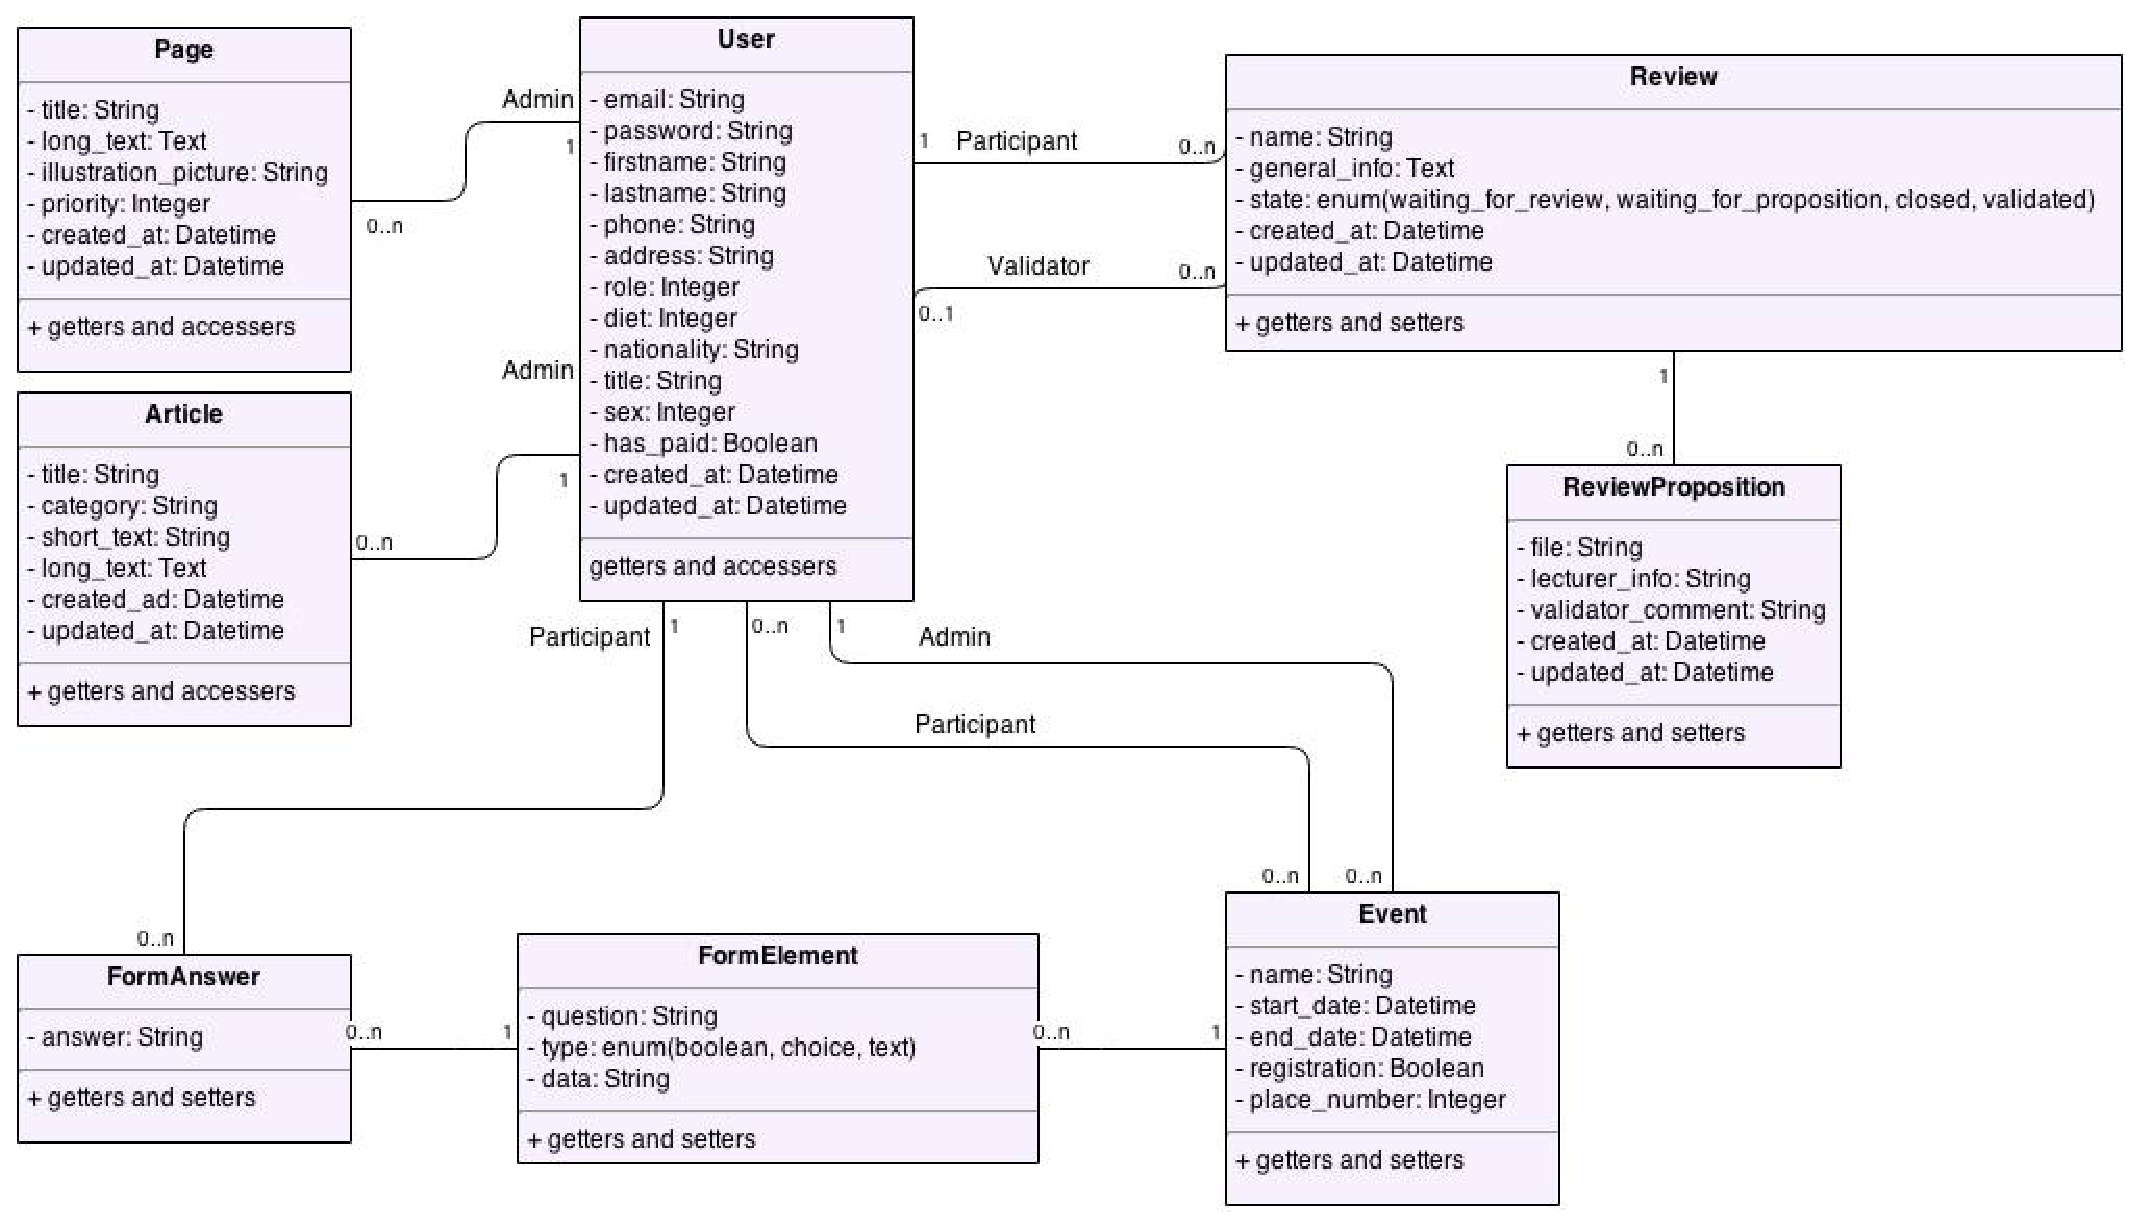
\includegraphics[width=15cm]{fig/uml-models}
   \caption{\label{uml} Diagramme \textit{UML} des modèles}
\end{figure}
Nous utilisons un ORM (Object-Relational Mapping), qui permet d'abstraire notre base de donnée. Ainsi la base de données est générée à partir de nos Modèles. Nous pouvons aisément passer d'une base de donnée sqlite, à une base MySQL ou encore PostgreSQL.

Nous avons donc réalisé un diagramme \textit{UML} de nos modèles.

\subsection{Technologies utilisées}
Le choix des technologies a été fait dans le but de créer un projet léger, et simple à mettre en place. 
\paragraph*{Ruby et Sinatra} Nous avons choisi d'utiliser le langage ruby en concert avec le framework Sinatra. Ce dernier est un DSL (Domain Specific Language), et est plus léger que d'autres gros frameworks comme \textit{Ruby on Rails}. Grâce à leur forte modularité, nous avons pu réutiliser de nombreux composants de base de \textit{Ruby on Rails}. 

\paragraph{SGBD}
Nous utilisons un SGBD relationnel à travers l'utilisation de l'ORM \textit{Activerecord}. Pour les développements, nous avons choisi d'utiliser une base de donnée \textit{sqlite3}, plus facile de configuration. Cependant, en changeant les paramètres, il est très facile de se connecter à une base \textit{MySQL} ou \textit{PostgreSQL}.

\paragraph{Frontend}
Afin d'uniformiser l'apparence du site web sur tous les navigateurs, de réaliser facilement un site web responsive et de minimiser les développements en CSS, nous avons choisi d'utiliser le framework \textit{Bootstrap}. Ce dernier livre aussi quelques élèments d'interfaces, très appréciés pour leur clarté.

\subsection{Organisation du projet}
Pour le projet, nous avons décidé de ne pas nous précipiter et de d'abord fixer les bases du projet. Lors de réunions effectuées entre membre du groupe, nous avons réfléchi durant le premier semestre aux technologies utilisées, mais aussi à l'organisation que nous suivrions durant le reste du projet. 

Nous avons choisi la méthode Agile comme méthode de travail. Nous devions donc poser différentes deadlines et présenter régulièrement notre travail à l'encadrant. Les différentes dates de rendu ont été placées afin d'avoir une base de travail convenable, et que chacun puisse s'y retrouver dans le travail à effectuer. Les différentes étapes furent les suivantes :

\begin{itemize}
\item Gestion des articles et des pages.
\item Gestion des événements et des utilisateurs.
\item Gestion des résumés et des paramètres du site.
\item Diverses améliorations.
\end{itemize}


\bigbreak
Il fut donc décidé d'utiliser \textit{GitHub}, un gestionnaire de version, afin de travailler tous sur le même projet mais chacun de son côté. Nous pouvions ainsi développer en local sur nos ordinateurs personnels, puis envoyer nos modifications sur le serveur commun.

D'autres fonctionnalités de \textit{GitHub} ont également été très utiles comme les \textit{Milestones} ou les \textit{issues}. Les premières permettent de poser une date de rendu de travail. Les \textit{issues} quant à elles nous permettaient de préciser différents soucis dans la construction ou le développement du site, ou de détailler les fonctionnalités à ajouter au site. Par exemple, pour les résumés, il a été décidé dès le début de créer un formulaire dans la partie profil utilisateur, d'obliger les fichiers à être au format pdf, et bien d'autres précisions concernant le développement.

@TODO:JEAN

\section{Développement des fonctionnalités}

\subsection{CMS}
L'une des premières fonctionnalités ajoutées furent les Articles et les Pages. Il s'agissaient de permettre la création, la modification et la suppression d'articles et de pages sans toucher une ligne de code. Pour la mise en place d'un système de CRUD (Create, Read, Update, Delete), nous avons travaillé chacun de notre côté afin d'assimiler les bases de Sinatra, de Ruby, d'HTML et de Bootstrap lorsque cela était nécessaire. Nous avons ainsi développé ces Pages et Articles dont la gestion est très semblable.

Après avoir ajouté les tables liées dans la base (tables articles et pages), il fallait d'abord créer un formulaire Web afin de rentrer les informations de la page ou de l'article. Les informations entrées sont ensuite utilisées pour la création d'un élément Article ou Page dans la base.

Suite à la création de la page, il était nécessaire d'avoir un formulaire afin de modifier la page ou l'article aisément. Dans la partie administration, les anciennes informations sont donc affichées et il est possible d'en entrer de nouvelles. Celles-ci permettront la mise à jour de l'élément sélectionné. La page ou l'article ont ensuite été liés à des boutons permettant de les supprimer. 

Il faut ensuite afficher ces pages ou articles. Lors d'une requête au serveur, les informations de la base de données sont envoyés à l'utilisateur et forment un article ou une page sur le navigateur.

\subsection{Évènements}
Les événements comportent trois aspects : la description de l'événement, la gestion de l'inscrition à l'événement, et la gestion des statistiques qui permettent de télécharger un fichier Excel, qui résumera toutes les inscriptions. 

Nous avons séparé le travail en petites étapes, construisant tout d'abord une base, puis en la complexifiant peu à peu. 

\medbreak
%\subsection*{La création des événements}

La première étape consiste en la création du \textit{CRUD} de l'événement. Cette étape est plutôt simple, puisqu'un événement n'est en lui même qu'un article avec quelques colonnes en plus : les dates de début et de fin de l'événement, le nombre limite de place, et l'activation des inscriptions. 

\medbreak
%\subsection*{La création du formulaire d'inscription}
Une fois le \textit{CRUD} de l'événement terminé, nous y avons ajouté la possibilité de créer un élément de formulaire. En effet, lorsque l'utilisateur s'inscrit à l'événement, on souhaite qu'il puisse remplir un formulaire pour ajouter des informations complémentaire (imaginons qu'un événement soit en hauteur, il peut être utile de savoir si l'utilisateur à le vertige\dots). 

Cette création est légèrement plus complexe que la création d'un article. Nous avons recontré une grosse difficulté ici : l'élément doit être relié à un événement. Il s'agit donc d'une relation \textit{many to one}. \textit{Activerecord} simplifier normalement ce processus. Cependant, la configuration n'a pas été correctement effectuée dans un premier temps. Il fallait alors écrire une grande partie des requêtes \textit{SQL} à la main. Cela a été une légère perte de temps, puisqu'il a fallu, quelques jours plus tard, corrigé cette maladresse. 

\medbreak
%\subsection*{La gestion des inscriptions}
Lorsque les éléments de formulaires furent correctement configurés,  nous avons implémenté l'inscription à un événement. Celle ci utilise également des relations \textit{SQL}, cependant la technologie nous étais connue à ce moment. Cette partie a donc été relativement rapide. 

Deux éléments sont a vérifié : l'utilisateur doit bien remplir les différents champs, et le site doit vérifier que le nombre limite de place n'a pas été dépassé.
\medbreak
%\subsection*{La gestion des statistiques}
Par la suite, nous avons mis en place la gestion des statistiques. 
Cette partie à également été plutôt rapide à produire. L'administrateur peut visualiser les statistiques de deux manières différentes (soit sur Excel, soit directement sur le site web). Nous avons donc décidé de créer un tableau ruby, résumant toutes les informations. Ce tableau peut ensuite être, soit affiché dans le site, soit exporté en fichier \textit{.xls}. 

C'est la seule partie du projet ou nous avons utilisé pleinement le langage Ruby. Malgré les conventions de nommage différentes de celle habituel (l'instance actuelle de l'objet s'appelle \verb!self!, et pas \verb!this! comme dans certains langage, ... ), l'utilisation d'un langage orienté objet nous est plutôt familière.   

\subsection{Utilisateurs}

Même si aux premiers abords, la gestion des utilisateurs peut sembler simple, elle recèle quelques subtilités. De plus, certaines informations étant confidentielles, il est important de les protéger correctement.

\subsubsection{Inscription / Connexion}

L'inscription et la connexion de l'utilisateur se font via un formulaire. Nous avons choisi l'email comme identifiant. 

La connexion est gérée via l'utilisation de sessions côté serveur. Afin de vérifier les identifiants fournis, un hash est généré à partir du mot de passe fourni et comparé à celui stocké en base de donnée

L'inscription se cantonne à créer un utilisateur en base de donnée, puis passe la main à la validation de l'email.

\subsubsection{Validation de l'email}

La validation de l'email se fait via l'envoi d'un email à l'adresse indiquée afin de vérifier que cette dernière est bien correcte et appartient bien à l'utilisateur. Ce dernier n'a plus qu'à cliquer sur un lien, et son compte sera validé. Afin d'améliorer l'expérience utilisateur, ce dernier est aussi authentifié. 

Côté serveur, un jeton est généré pour l'utilisateur, à usage unique. A partir de ce dernier et de l'email de l'utilisateur, un lien est généré, et envoyé par email. Lors du clic sur le lien, si les informations correspondent, l'utilisateur passe authentifié et est automatiquement connecté pour cette session. Le jeton est alors détruit.

\subsubsection{Sécurité}

Tous d'abord, les mots de passes sont hashés et salés dynamiquement. Tout d'abord, le hash est une fonction injective, et ne permet donc pas de retrouver le mot de passe depuis ce dernier. De plus, le fait de saler le mot de passe permet d'empêcher la personne malveillante de retrouver le mot de passe à partir d'un rainbow table, ni même d'en générer ou encore de réaliser des suppositions sur le mot de passe. En effet, deux utilisateurs ayant le même mot de passe auront un hash différent grâce au salage dynamique.

Enfin, une fois authentifié, l'utilisateur est géré via une session, les informations sont donc stockées côté serveur et ne peuvent donc pas être modifiées par la personne. Ce qui serait le cas si elles étaient stockées directement dans le cookie.

Plusieurs rôles sont définis : Non authentifié, Compte Non validé, Utilisateur, Modérateur et Administrateur. Chaque page peut être restreinte à un rôle particulier.

\subsubsection{Récupération de mot de passe}

La récupération de mot de passe fonctionne sensiblement pareil que la validation par email. Un jeton est généré pour l'utilisateur, qui lui est envoyé par mail et permet à ce dernier de se connecter sans entrer son mot de passe. Ce dernier est détruit à l'utilisation. Mais l'utilisateur peut changer son mot de passe durant cette session.

\subsection{Candidatures}

Les Reviews sont les résumés envoyés par les inscrits qui souhaitent participer à la conférence. Il faut donc récupérer des fichiers soumis sur le site. Une des difficultés est donc le stockage de ces fichiers. En effet ceux-ci doivent être accessible facilement par le serveur, pour l'affichage ultérieur, mais pas par un utilisateur lambda. Sinatra et Ruby permettent la sauvegarde des fichiers envoyés. 


\bigbreak
Cependant, il a d'abord fallu créer les tables \textit{reviews} et \textit{reviewpropositions} dans la base de donnée. \textit{Reviews} contient le nom du participant, le nom de la conférence, l'état de l'inscription et est lié aux reviewpropositions. Ceux-ci sont crées à chaque nouvelle soumission de résumé. Ils contiennent le lien vers le fichier, un commentaire du participant expliquant la proposition et le lien vers la review liée. 

Ici, le lien entre les \textit{reviews}, \textit{reviewpropositions} et \textit{users} ont été difficiles à mettre en place. Il a fallu créer des associations entre les différentes tables. Après de nombreux essais, recherches et tests, les liens en dur ont été changés en \textit{references} entre les tables. 


\bigbreak
Lorsque les tables furent crées et la base de données migrée, est arrivé le problème de la sauvegarde des fichiers. Le choix fut fait de stocker les fichiers à la racine du projet et de stocker dans la base de donnée les hash MD5 des fichiers. Il s'agit d'une chaine de caractère générée selon un algorithme. Elle est différente pour chaque fichier et permet donc de les différencier dans la base. En effet, stocker le nom serait une très mauvaise idée si deux fichiers se trouvaient à avoir le même nom. 

La soumission des résumés par les utilisateurs fut donc ajoutée dans la partie profil


\subsection{Paramètres}

Nous avons voulu créer une plateforme de gestion de conférence assez ouverte. Nous voulons donc que cette dernière puisse être réutilisable pour d'autres évènements, c'est pourquoi de nombreuses données peuvent être modifiées.

Entre autre les informations de base du site : nom, slogan, couverture. Mais aussi des informations de paiement, le serveur de mail utilisé...

\section{Qualité logiciel}

La qualité logiciel a été un point clé du développement de notre application web, et ce dès le début. En étant strict à ce niveau là, nous n'avons pas rencontré de problèmes particuliers lorsque la taille du projet a commencé à augmenter.

\subsection{Gestionnaire de version}

Nous avons choisi \textit{git}, gestionnaire de version de dernière génération et actuellement le plus utilisé. Nous avons pu profiter de toutes ses fonctionnalités, avec entre autre les tags et les branches. Nous nous sommes basés sur un modèle existant et éprouvé\cite{nvie} et l'avons adapté à nos besoins.

\subsection{Tests unitaires}

Nous avons testé unitairement l'ensemble des classes que nous utilisions : nos modèles ainsi que toutes nos classes appartenant à notre business layer. 

Nous n'avons pas pu tester nos controllers unitairement, car en ayant fais le choix de Sinatra, un DSL, ces derniers ne sont pas testables.

\subsection{Tests fonctionnels}

Les tests fonctionnels sont des scénarios types, pour tester le comportement de notre application dans son ensemble.

En ayant fais le choix de \textit{Capybara}, nous pouvons à travers son API unique, lancer nos tests sur une grande variété de plateformes. En effet, par défaut les tests fonctionnels se font sans interface graphique, grâce au driver \verb!rack_test! qui ne lance pas de navigateur et se contente de vérifier le html généré. 

Mais sans modifier nos tests, nous pouvons lancer ces derniers avec \textit{Selenium-Webdriver}, qui lance le navigateur de notre choix et simule les clics de souris et les entrées claviers.

\subsection{Intégration continue}

L'intégration continue permet de s'assurer de la viabilité de notre projet au cours de son développement.

En effet, à chaque commit \textit{Travis} lance un build. Pour chaque build, \textit{Travis} créer une nouvelle machine virtuelle, totalement vierge. Puis, il installe les dépendances, configure l'environnement et lance les tests.

Ainsi, nous nous assurons que pour un commit donné, notre application est bien pleinement compatible avec un environnement donné et clairement défini.

Dans le cas d'un échec de build, les collaborateurs du projet reçoivent un mail les alertant de l'erreur, ainsi qu'un compte-rendu du build.

Nous pouvons alors sereinement déployé notre application à n'importe quel moment.

Enfin \textit{Travis} permet de créer des matrices de build, qui permettent de tester le projet avec des configuration différentes. Par exemple 4 versions de ruby différentes et 3 SGBD différents. \textit{Travis} lancera alors 12 builds.

\subsection{Revue de code automatique}

La revue de code automatique permet à notre équipe d'acquérir les bons réflexes et de s'améliorer au fur et à mesure du développement de l'application.

Cela permet aussi d'améliorer sa maintenabilité.

\textit{Codeclimate} calcule aussi la couverture de tests de l'application, afin d'avoir un aperçu des fonctions testées et des fonctions qui ne sont pas testées.

\section{Déploiement}

Nous n'avons pas encore eu l'occasion de déployer notre projet en production, mais avons un serveur de démo (UAT, User Acceptance Testing).

Il est d'ailleurs actuellement accessible à l'URL suivante : http://suzanne.deuxfleurs.fr

Nous avons choisi un conteneur LXC pour le compartimenter du reste du système, avec une distribution Debian stable.

Nous recommandons l'utilisation du serveur web thin en lieu et place du serveur de développement webrick. En effet, thin est plus optimisé. De plus, il est possible de mettre en place un reverse proxy, comme nginx ou varnish devant le serveur ruby, qui peut servir les fichiers statiques directement sans avoir à passer par notre serveur, nécessairement plus lent.

Dans le cas d'une utilisation professionnelle, il est aussi fortement recommandé d'utiliser une connexion chiffrée avec un certificat valide (https), afin d'éviter la transmission d'informations sensibles en clair. 

\section{Conclusion} 
 
Le développement de cette étude pratique nous a permis de nous mettre en situation d’une gestion de projet, étape essentiel dans la vie d’un élève-ingénieur. Nous avons expérimenté le développement en groupe, mais nous avons pu également aborder la relation client.

Nous avons commencé par comprendre les besoin de notre encadrant puis  de trouver les technologies adaptés. Nous avons aussi collaboré pour implémenter chaque fonctionnalité une à une, en s’assurant qu’elles correspondent à ce qu’il attendais.

La séparation des tâches nous a permis de nous focaliser chacun sur notre travail à réaliser, et aussi d’optimiser le temps d’apprentissage, chacun apprend ce dont il a besoin.

Dans le cadre d’un prolongement du développement du projet, il est envisageable d’implémenter une interface dynamique grâce à Javascript.
Nous avons construit un système complexe composé de plusieurs technologies, tout en vérifiant en permanence que ce que l’on développe correspond au besoin de notre encadrant. 



\bibliography{biblio}


\end{document}

%%%%%%%%%%%%%%%%%%%%%%%%%%%%%%%%%%%%%%%%%%%%%%%%%%%%%%%%%%%%%%%%%%%%%%%%%%%%%%%
